\documentclass[12pt]{article}
\usepackage{amsmath}
\usepackage{amssymb}
\usepackage[letterpaper,top=1in,bottom=1in,left=0.75in,right=0.75in,centering]{geometry}
%\usepackage{fancyhdr}
\usepackage{enumerate}
%\usepackage{lastpage}
\usepackage{multicol}
\usepackage{graphicx}

\reversemarginpar

%\pagestyle{fancy}
%\cfoot{}
%\lhead{Math 1560}\chead{Test \# 1}\rhead{May 18th, 2017}
%\rfoot{Total: 10 points}
%\chead{{\bf Name:}}
\newcommand{\points}[1]{\marginpar{\hspace{24pt}[#1]}}
\newcommand{\skipline}{\vspace{12pt}}
%\renewcommand{\headrulewidth}{0in}
\headheight 30pt

\newcommand{\di}{\displaystyle}
\newcommand{\abs}[1]{\lvert #1\rvert}
\newcommand{\len}[1]{\lVert #1\rVert}
\renewcommand{\i}{\mathbf{i}}
\renewcommand{\j}{\mathbf{j}}
\renewcommand{\k}{\mathbf{k}}
\newcommand{\R}{\mathbb{R}}
\newcommand{\aaa}{\mathbf{a}}
\newcommand{\bbb}{\mathbf{b}}
\newcommand{\ccc}{\mathbf{c}}
\newcommand{\dotp}{\boldsymbol{\cdot}}
\newcommand{\bbm}{\begin{bmatrix}}
\newcommand{\ebm}{\end{bmatrix}}                   
                  
\begin{document}


\author{Instructor: Sean Fitzpatrick}
\thispagestyle{empty}
\vglue1cm
\begin{center}

{\bf MATH 2565 - Tutorial \#5 Solutions}
\end{center}

\textbf{Assigned problems:}


 \begin{enumerate}



 \item Find the volume of the solid $S$ whose base is the region of the $xy$-plane bounded by $y=x^2$ and $y=2-x^2$, and whose cross-sections parallel to the $y$-axis are squares.
 
\medskip

\begin{multicols}{2}
\begin{center}
 \includegraphics[width=0.45\textwidth]{WS4-2a.png}
\end{center}

The base of each square has width $y_1-y_2 = 2-x^2-x^2 = 2-2x^2$, so the cross-sectional area is $A(x) = (2-2x^2)^2 = 4-8x^2+4x^4$. The two parabolas intersect when $x=\pm 1$, so the volume is
\begin{align*}
 V=\int_{-1}^1A(x)\,dx &= \int_{-1}^1(4-8x^2+4x^4)\,dx \\&= \frac{64}{15}.
\end{align*}
 \end{multicols}
 
 \item Find the volume of the solid $S$ generated when the region bounded by the curves $y^2=x$ and $x=2y$ is revolved around the $y$-axis.
 
 \medskip
 
 \begin{multicols}{2}
  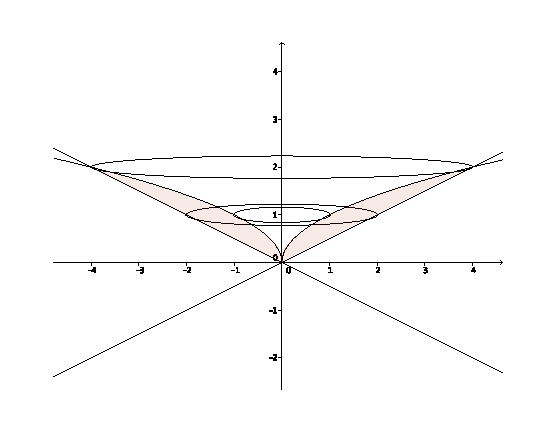
\includegraphics[width=0.45\textwidth]{WS4-2d}


From the diagram above we see that we have a solid whose cross-sections parallel to the $x$-axis are washers, with inner radius $r_{in}(y)=y^2$, and outer radius $r_{out}(y)=2y$, with $0\leq y\leq 2$. The cross-sectional area is
\begin{align*}
 A(y) &= \pi r_{out}(y)^2-\pi r_{in}(y)^2 \\&= \pi (4y^2-y^4).
\end{align*}
The volume is therefore
\begin{align*}
 V &= \int_0^2A(y)\,dy\\& = \pi \int_0^2 (4y^2-y^4)\,dy\\& = \pi\left.\left(\frac{4}{3}y^3-\frac{1}{5}y^5\right)\right|_0^2\\& = \frac{64\pi}{15}.
\end{align*}
\end{multicols}

\pagebreak

 \item Use the shell method to find the volume of the solid generated by revolving the region bounded by $y=x$ and $y=\sqrt{x}$ about the $x$-axis.
 
 \medskip
 
 \begin{multicols}{2}
\begin{center}
 \includegraphics[width=0.45\textwidth]{WS5-6.png}
\end{center}

The graphs $y=x$ and $y=\sqrt{x}$ can be rewritten as $x=y^2$ and $x=y$. Using cylindrical shells, the radius of each cylinder is $r=y$, and the height is $h = y-y^2$, so the surface area of each shell is $2\pi y(y-y^2)$, and the volume is
\[
 V = \int_0^1 2\pi (y^2-y^3)\,dy = \frac{\pi}{6}.
\]

 \end{multicols}
 
 \item Find the length of the curve $y=\dfrac{1}{12}x^3+\dfrac{1}{x}$, for $x\in [1,4]$.

\medskip

Arc length is given by $L=\int_a^b\sqrt{1+f'(x)^2}\,dx$, so we first compute
\begin{align*}
 1+(y')^2 & = 1+ \left(\frac{1}{4}x^2-\frac{1}{x^2}\right)^2 = 1+\left(\frac{x^4-4}{4x^2}\right)^2\\
& = 1+\frac{x^8-8x^4+16}{16x^4} = \frac{16x^4+x^8-8x^4+16}{16x^4}\\
& = \left(\frac{x^4+4}{4x^2}\right)^2.
\end{align*}
Thus, 
\[
 L = \int_1^4 \sqrt{\left(\frac{x^4+4}{4x^2}\right)^2}\,dx = \int_1^4 \left(\frac{x^2}{4}+\frac{1}{x^2}\right)\,dx = 6.
\]

\end{enumerate}

\pagebreak

\textbf{Additional practice} 
\begin{enumerate}
 \item Find the volume of a right circular cone whose height is 12 and base radius is 4.
 
 \medskip

\begin{multicols}{2} 
\begin{center}
  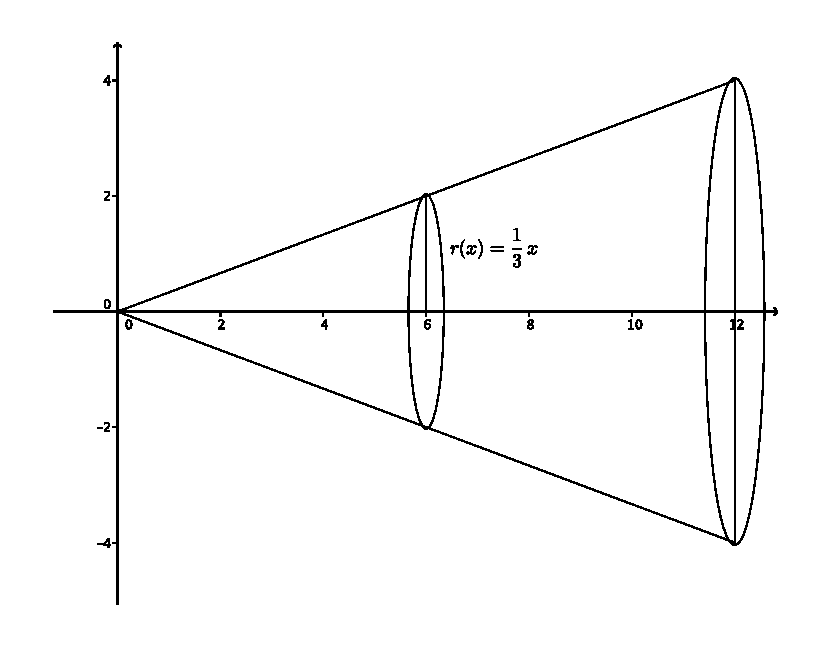
\includegraphics[width=\columnwidth]{WS4-2b}
\end{center}

To keep things simple, we orient our cone with vertex at the origin and base at $x=12$, so that the radius as a function of $x$ is given by $r(x)=\frac{1}{3}x$. (If you put the base along the $y$-axis the radius is $4-\frac{1}{3}x$ and the integral is a lot more complicated, although of course the answer works out to be the same.)
 Cross-sections of the cone are disks, with cross-sectional area $A(x) = \pi r(x)^2$, so the volume is
 \end{multicols}
\[
 V = \int_0^{12}A(x)\,dx = \pi\int_0^{12}\frac{x^2}{9}\,dx = \left.\frac{\pi}{27}x^3\right|_0^{12} = 64\pi.
\]

 \item Find the volume of the solid generated by revolving the region bounded by $y=x^2$, $x=1$, and $y=0$ about the $x$-axis.
 
 \medskip
 
 \begin{multicols}{2}
 \begin{center}
 \includegraphics[width=\columnwidth]{WS5-1.png}
\end{center}

Using the disc method, our cross-sectional area is $A(x) = \pi y^2 = \pi(x^2)^2 = \pi x^4$. The volume is therefore
\[
 V = \int_0^1 \pi x^4\,dx = \frac{\pi}{5}.
\]
\end{multicols}

 \item Find the volume of the solid generated by revolving the region bounded by $y=\sqrt{x}$, $y=1$, and $x=0$ about
 \begin{enumerate}
 \item the $x$-axis

\medskip

\begin{multicols}{2}
 \begin{center}
  \includegraphics[width=0.8\columnwidth]{WS5-2a.png}
 \end{center}
 \begin{center}
  \includegraphics[width=0.8\columnwidth]{WS5-2b.png}
 \end{center}
\end{multicols}
Using washers, our cross-sectional area is $A(x) = \pi(1)^2-\pi(\sqrt{x})^2 = \pi(1-x)$, so the volume is
\[
 V = \int_0^1\pi(1-x)\,dx = \frac{\pi}{2}.
\]
If we use cylindrical shells instead, each shell has surface area $A(y) = 2\pi r(y)h(y) = 2\pi y(y^2) = 2\pi y^3$, so the volume is
\[
 V = \int_0^1 2\pi y^3\,dy = \frac{\pi}{2}.
\]

 \item the $y$-axis

 
 \medskip
 
 The resulting solid is identical to the one in problem 1, except that it's revolved around the $y$-axis instead of the $x$-axis, and the volume is again $\pi/5$.
\end{enumerate} 

 \item Find the volume of the solid generated by revolving the region bounded by $x=y-y^2$ and $x=0$ about the $y$-axis.
 
 \medskip
 
 \begin{multicols}{2}
\begin{center}
 \includegraphics[width=0.5\textwidth]{WS5-4.png}
\end{center}

Using discs, we have cross-sectional area $A(y) = \pi(y-y^2)^2$, so the volume is
\[
 V = \int_0^1 \pi(y^2-2y^3+y^4)\,dy = \frac{\pi}{30}.
\]
\end{multicols}

\pagebreak

 \item Find the volume of the solid generated by the region bounded by $y=4-x^2$ and $y=0$, when rotated about

\begin{enumerate}
 \item the $x$-axis.

\medskip
\begin{multicols}{2}
 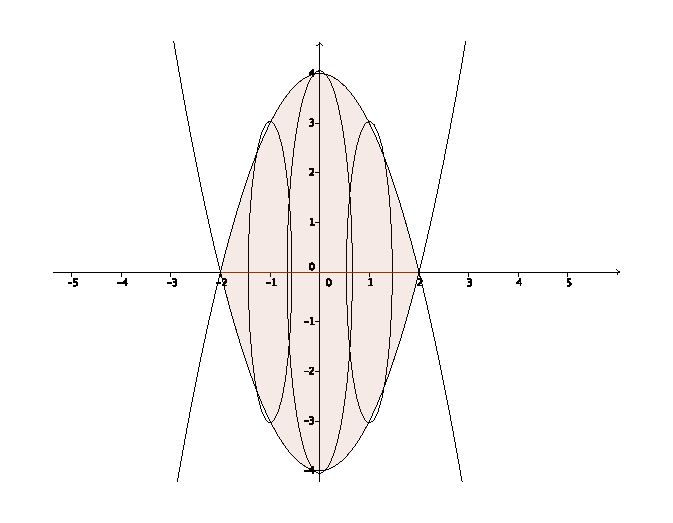
\includegraphics[width=0.45\textwidth]{WS4-2ci}


We have a solid of revolution, so cross-sections are disks, with radius $r(x)=4-x^2$. The cross-sectional area is therefore $A(x)=\pi(4-x^2)^2$, and the volume is given by
\[
 V = \int_{-2}^2A(x)\,dx = \pi\int_{-2}^2(16-8x^2+x^4)\,dx.
\]
Since the integrand is even, we have
\end{multicols}
\[
 V=2\pi\int_0^2(16-8x^2+x^4)\,dx = 2\pi\left.\left(16x-\frac{8}{3}x^3+\frac{1}{5}x^5\right)\right|_0^2 = \frac{512\pi}{15}.
\]

 \item the line $y=-1$.
 
 \medskip

\begin{multicols}{2}
 
  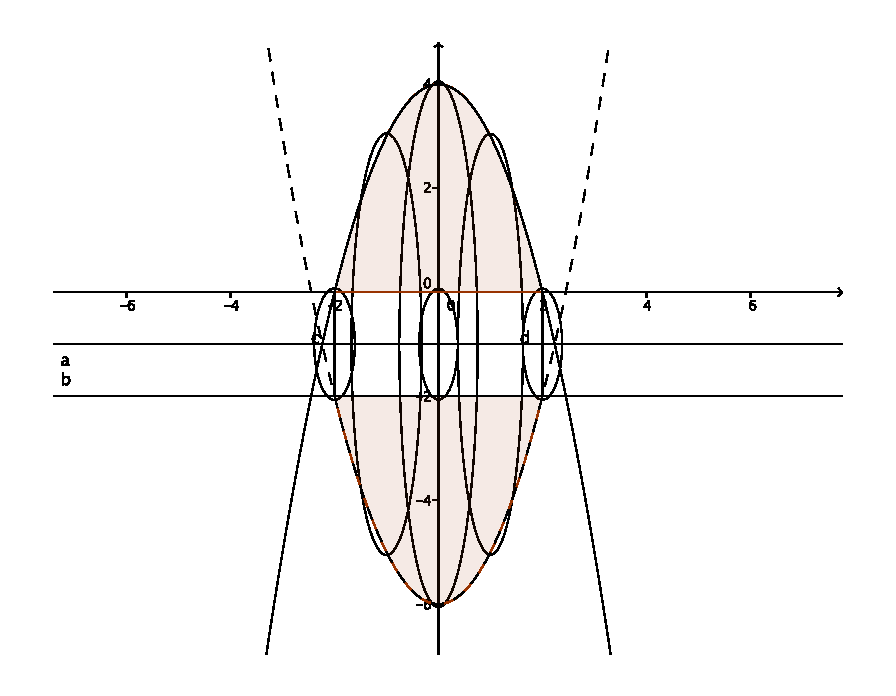
\includegraphics[width=0.45\textwidth]{WS4-2cii}


We have a solid of revolution, but since the axis of rotation is one unit away from the bottom of the region being revolved about the axis, cross-sections are washers. The inner radius is 1, and the outer radius is $r(x)=y(x)+1=5-x^2$, so the cross-sectional area is
\end{multicols}
\[
 A(x) = \pi r_{out}(x)^2-\pi r_{in}(x)^2 = \pi(5-x^2)^2-\pi(1)^2 = 24-10x^2+x^4.
\]
Noting that $A(x)$ is an even function, we have

\[
 V = \int_{-2}^2A(x)\,dx = 2\int_0^2(24-10x^2+x^4)\,dx = \pi\left.\left(24x-\frac{10}{3}x^3+\frac{1}{5}x^5\right)\right|_0^2 = 16\pi\left(\frac{26}{15}\right).
\]

 \item the line $x=2$.
 
 \medskip
 
  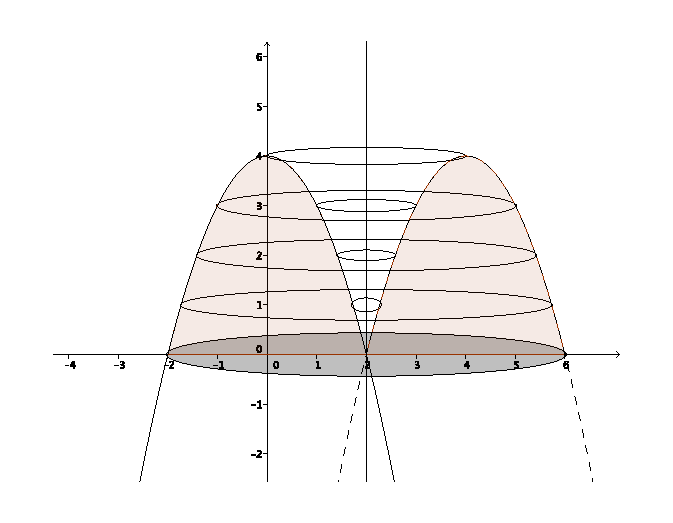
\includegraphics[width=0.75\textwidth]{WS4-2ciii}


This time we're revolving about an axis parallel to the $x$-axis, so we have to solve for $x$ in terms of $y$. We find $x=\pm \sqrt{4-y}$, where the positive root corresponds to the right half of the parabola, and the negative root to the left half. The cross-sections are again washers if we slice horizontally. The inside of the washer corresponds to the right of the parabola, and the outside of the washer corresponds to the left of the parabola, so the inner and outer radii of the washer are given by
\[
 r_{in}(y) = 2-x = 2-\sqrt{4-y} \quad \text{ and } \quad r_{out}(y) = 2-(-\sqrt{4-y}) = 2+\sqrt{4-y}.
\]
The cross-sectional area is therefore
\[
 A(y) = \pi r_{out}(y)^2-\pi r_{in}(y)^2 = \pi (2+\sqrt{4-y})^2 - \pi (2-\sqrt{4-y})^2 = 8\pi\sqrt{4-y},
\]
so the volume is given by
\[
 V = \int_0^4 A(y)\,dy = 8\pi\int_0^4 (4-y)^{1/2}\,dy = \left.-\frac{16\pi}{2}(4-y)^{3/2}\right|_0^4 = \frac{128\pi}{3}.
\]


\end{enumerate}
\pagebreak

 \item Find the volume of the solid generated by revolving the region bounded by $x=y-y^2$ and $x=0$ about the $y$-axis.
 
 \medskip

\begin{multicols}{2} 
 \begin{center}
 \includegraphics[width=0.45\textwidth]{WS5-4.png}
\end{center}

Using discs, we have cross-sectional area $A(y) = \pi(y-y^2)^2$, so the volume is
\[
 V = \int_0^1 \pi(y^2-2y^3+y^4)\,dy = \frac{\pi}{30}.
\]
\end{multicols}

 \item Use the shell method to find the volume of the solid generated by revolving the region bounded by $y=6x-2x^2$ and $y=0$, about the $y$-axis.

\medskip

\begin{center}
 \includegraphics[width=0.5\textwidth]{WS5-5.png}
\end{center}

Note that $6x-2x^2=2x(3-x)$, so the graph $y=6x-2x^2$ intersects the $x$-axis when $x=0$ and $x=3$. Using shells, the height of each cylinder is $h = y = 6x-2x^2$, and the radius is $r=x$, so the surface area of each shell is $2\pi x(6x-2x^2)$, and the volume is
\[
 V = \int_0^3 2\pi x(6x-2x^2)\,dx  = 27\pi.
\]
\end{enumerate}


%\thispagestyle{empty}




\end{document}